\section{Bucketsort}
O Bucketsort é um algoritmo de ordenação descrito por John W. Tukey em 1944. Ele se baseia na distribuição dos elementos em diferentes grupos, chamados ``buckets'', cujos conteúdos são ordenados individualmente. Por fim, os buckets são concatenados, resultando em um vetor ordenado.

\begin{figure}[H]
\Caption{\label{fig:buckets}Ilustração do intervalo correspondente a cada bucket, em que $B_i$ representa o $i$-ésimo bucket e $M$ é o maior elemento que pode existir no vetor.}
\centering
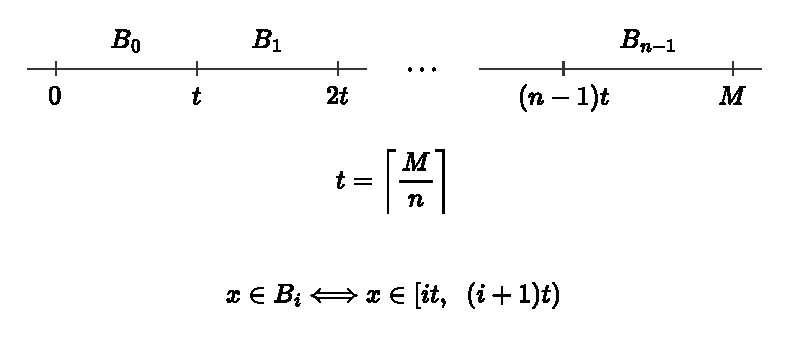
\includegraphics[scale=1.0]{figuras/pdf/buckets.pdf}
\Fonte{Elaborado pelo autor.}
\end{figure}

Caso os elementos do vetor de entrada estejam distribuídos de forma uniforme no intervalo $[0, M]$, é esperado que cada bucket contenha uma quantidade constante de elementos, de modo que o algoritmo Bucketsort execute em tempo linear. No entanto, não se sabe previamente quantos elementos cada bucket armazenará durante a execução. Por isso, cada bucket foi implementado como uma estrutura de crescimento dinâmico, utilizando listas ligadas. Além disso, o método InsereOrdenado foi desenvolvido de forma semelhante ao algoritmo Insercao.

\lstinputlisting[language=C]{codigos/lin/2_bucketsort.txt}
